\documentclass[11pt]{article}
\usepackage{amsmath}
\usepackage{amsfonts}
\usepackage{graphicx}
\usepackage[margin = 1.3 in]{geometry}
\usepackage{pgfplots}
\usepackage{tikz}
%opening
\title{Electric Fields and Electric Potential}
\author{Andreas Badea}

\begin{document}

\maketitle
\begin{center}
	\begin{tabular}{l r}
		Partners: & Eashwar Mahadevan \\
		& Alex Hoerler \\
		Date Performed: & January 11, 2018 \\ % Date the experiment was performed
		Instructor: & Dr. Bradley Miller % Instructor/supervisor
	\end{tabular}
\end{center}

\section{Introduction}
Coulomb's Law describes the force acting between statically charged particles.
\begin{equation}
\mathbf{F} = \frac{k q_1 q_2}{r^2} \hat{\mathbf{r}}
\end{equation}
That is, if two charged particles were to be placed together, at a distance \(r\) from each other. They would feel a force proportional to the product of their charges and inversely proportional to the square of the distance between them. This relation conveniently allows one to describe the force acting on a pair of particles, but often is is convenient to describe the forces in an alternative way. 
\\\\
Consider gravity.

\begin{equation}
\mathbf{F} = \frac{G m M}{r^2} \hat{\mathbf{r}}
\end{equation}
 Newton describes the force due to gravity in a remarkably similar way Coulomb: In this case proportional to the product of the masses and the inverse of the square of the distance. But when describing events on the surface of the earth, the mass of the object acted on need not be considered. One may simply discuss a constant acceleration. Effectively, by dividing both sides of the expression by the mass of the on may see a body as creating some sort of gravitational field of force per mass (acceleration) around it that exists with or without another body to act upon.
 
It is natural to do the same with electrostatic relationships as well. However, rather than dividing both sides by the mass, consider dividing by a charge. This allows us to consider each charged particle as creating electric field irrespective of any neighboring particles. This field is one of force per charge. That is the force acting on any charged particle within a field is equal to the product of the field and the particle's charge.

\begin{equation}
	\mathbf{F} = q \mathbf{E}
\end{equation}

This electric field, \(\mathbf{E}\), is simply a vector field generated by each particle.

\begin{equation}
\mathbf{E} = \frac{k_e q}{r^2} \mathbf{\hat{r}}
\end{equation}

When confronted with any vector field, particularly one that deals with forces it is natural to try and fit a potential function to it.  That is, to find some scalar function \(f\) such that \(\nabla f = \mathbf{F}\). Of course, this may only be done if the vector field is conservative, but this happens to be the case. This potential function would allow one to find the work to get from one point to another without the need of any line integrals and allow one to associate a potential energy to each point.

However, we would like to keep this in terms of an electric field and not a force. So we shift out perspective to find a function \(V\) such that \(\nabla V = \mathbf{E}\). This scalar field \(V\) is called the electric potential.  This field should represent energy per charge.

Visually one should be able to represent the electric field as a standard vector field. The electric potential could be visualized as a 3d graph, but is often more convenient to view it as a series of contours. Note that the contours will always be perpendicular to the field lines.
\begin{figure}[h]
	\begin{center}
	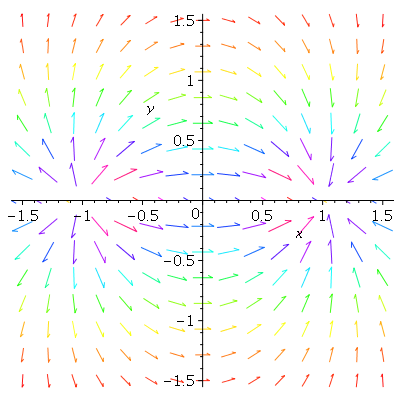
\includegraphics[width=2in]{field}
	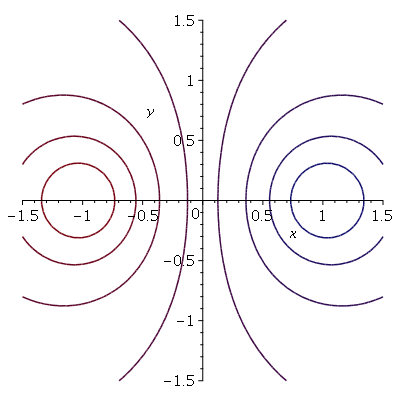
\includegraphics[width=2in]{cont}
	\end{center}
	\caption{Field Lines and Contours of Electric potential for a particular charge configuration (Dipole)}
\end{figure}

\section{Procedure}
An experiment was conducted to see that electric potential and dipole behave as posited by Coulomb's Law, and by their relationship as potential functions and gradients for one another. To do this, the electric potential difference was measured between various points. 
\subsection{Dipole Configuration}
In order to generate a dipole configuration, two small conductive dots were placed on the gridded paper. These two dots were placed at the 8 and 17 cm marks on the paper (9 cm apart). A small pin was placed into each of these dots. A power supply which outputted a constant 10 V was attached to the configuration. One of leads was attached to each of the pins on the paper. A digital multi-meter was then used to measure voltage differences across the paper. One end of the multimeter was attached to one end of the power supply while the other was attached to a small probe which was placed at various points along the paper. This measured the difference in voltage between the power supply and that particular point on the paper.

The voltage difference was measured at 1cm intervals along the horizontal lines on which the two points of charge fell. And Lines of equipotential were traced by moving the probe while attempting to keep the voltage difference constant.

\subsection{Alternative Configuration}
A similar procedure was followed for an alternative charge configuration. This charge configuration consisted of a small line of charge and lying opposite that line a teardrop shape of charge. Both were made of conductive ink. Once again equipotential were traced.


\section{Data}
The voltage difference between one of the poles and various points were measured and recorded. Among these points were the those on the line passing through the two points of charge. The paper was marked with a 1 cm grid and the two points of charge were placed at points 8 and 17.
\begin{figure}[h]
	\centering
	\caption{Voltage at points through horizontal axis }
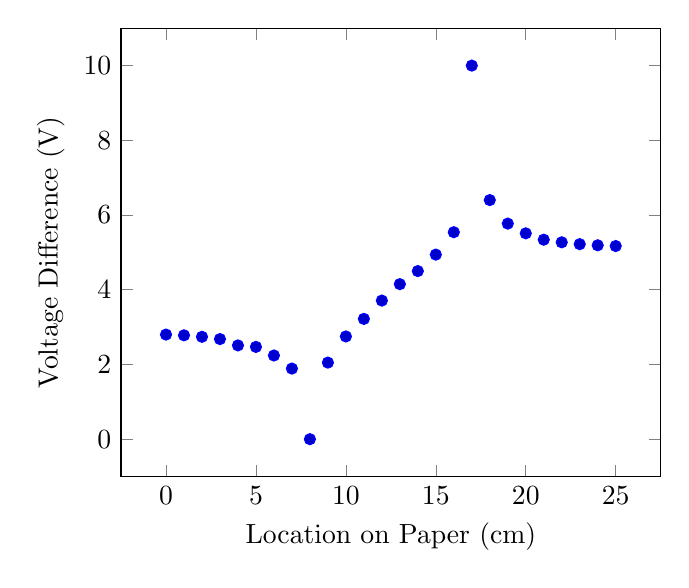
\begin{tikzpicture}
	\begin{axis}[xlabel={Location on Paper (cm)},
	ylabel = {Voltage Difference (V)}]
	\addplot+[only marks]
	table[]
	{
		x	y
		0	2.8
		1	2.78
		2	2.74
		3	2.68
		4	2.51
		5	2.47
		6	2.24
		7	1.89
		8	0
		9	2.05
		10	2.75
		11	3.22
		12	3.71
		13	4.15
		14	4.5
		15	4.94
		16	5.54
		17	10
		18	6.4
		19	5.77
		20	5.51
		21	5.34
		22	5.27
		23	5.22
		24	5.19
		25  5.17
	};
	\end{axis}
	\end{tikzpicture}
\end{figure}

The equipotential curves were also traced out for each of the configurations. See the attached page.
\section{Analysis}
One might attempt to fit a model for the electric potential of a dipole over the data collected. Doing this proves relatively simple. Consider a dipole with point charges \(q\) and \(-q\) respectively at points \(a\) and \(b\). We simply wish to find the electric potential at a point \(x\) on the line through the dipole. We begin by finding the electric field at \(x\). Recall that the electric field due to a point charge is
\begin{equation}
\mathbf{E} = \frac{k q}{r^2} \mathbf{\hat{r}}
\end{equation}
In this case, \(\mathbf{r}\) simply refers to the distance to the point charge. The distances between the point charges and \(x\) are simply \(|x-a|\) and \(|x-b|\). However, this is not the only \(\mathbf{r}\) based term in the expression. The force acts in the direction of \(\mathbf{r}\), \( \mathbf{\hat{r}} \). This we represent, somewhat more frustratingly with \(\mathrm{sgn}(x-a)\) and \(\mathrm{sgn}(x-b)\) where \(\mathrm{sgn}(x)\) is the sign function, returning 1 for positive values and -1 for negative inputs. Substituting these terms and summing the two relevant expressions (for each a and b). We are left with the rather unsatisfying result.
\begin{equation}
\mathbf{E} = \frac{k q}{(x-a)^2} \mathrm{sgn}(x-a) - \frac{k q}{(x-b)^2}\mathrm{sgn}{x-b}
\end{equation}
We are now left to find the potential function. Because this is in one dimension we must simply take a simple integral. Conveniently, this allows us to clean up our expression quite a bit. Recall that sign function is expressed (and occasionally defined) as the derivative of the absolute value function. This makes the integral relatively easy and leaves one with the much more satisfying potential function.

\begin{equation}
V = \frac{k q}{|x-a|} - \frac{k q}{|x-b|}
\end{equation}

One might even try to fit this curve to the data collected above. However, it requires some modification. There is no convenient way to separate the \(k\) and \(q\) parameters, which always appear in a pair, so it is convenient to replace it with a single parameter \(C\) which represents their product. Also, like with energy, with voltage only differences may be measured. Thus the fit will be offset by some constant \(V_0\) which represents the limit voltage difference measure as one gets arbitrarily far away from the dipole configuration. This value should also be the voltage at the exact middle of the dipole. Intuitively, its value should be the mean of voltage at the two poles.

\begin{equation}
V = \frac{C}{|x-a|} - \frac{C}{|x-b|} + V_0
\end{equation}

With these adjustments in mind one may fit a curve to the data collected.
\section{Conclusions}
\begin{figure}[h]
	\centering
	\caption{Voltage at points through horizontal axis: Dipole fit }
	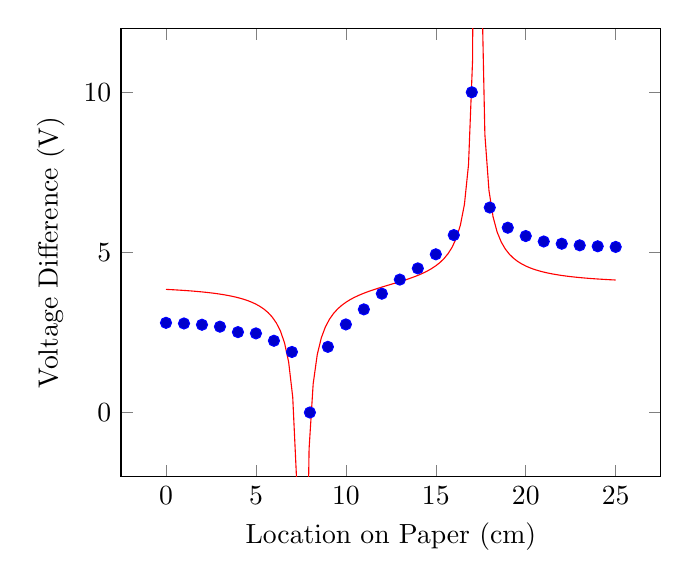
\begin{tikzpicture}
	\begin{axis}[xlabel={Location on Paper (cm)},
	ylabel = {Voltage Difference (V)},ymax=12,ymin=-2]
	\addplot+[only marks]
	table[]
	{
		x	y
		0	2.8
		1	2.78
		2	2.74
		3	2.68
		4	2.51
		5	2.47
		6	2.24
		7	1.89
		8	0
		9	2.05
		10	2.75
		11	3.22
		12	3.71
		13	4.15
		14	4.5
		15	4.94
		16	5.54
		17	10
		18	6.4
		19	5.77
		20	5.51
		21	5.34
		22	5.27
		23	5.22
		24	5.19
		25  5.17
	};
	\addplot[red,samples=111,domain=0:25] {-1.989/abs(x-7.582) + 1.989/abs(x-17.32) + 3.992};
	\end{axis}
	\end{tikzpicture}
\end{figure}

The fit is decidedly disappointing. One can clearly see that shape of the graph is generally correct, however we may clearly see quite a few short comings. The correlation of the graph is reasonably high at 0.913 but the RMSE is a rather elephantine 0.87 V. That means that on average we deviate from out predictions by nearly 9\%. Upon further examination of our graph we notice that we predict the potential to die away as we leave the dipole much more quickly than it truly does. Examining the parameters provides some clarity. The \(a\) and \(b\) parameters are found to be \(7.58 \pm 0.07\) cm and \(17.32 \pm 0.05\) cm respectively. Both relatively close to their true values of 8 and 17 cm. Percent errors are not particularly meaningful values to compare here, but the absolute error indicates that the predictions are off by a 0.42 and 0.32 cm respectively. The parameter for \(V_0\) indicates that the base voltage should have been the same as the middle value between the two nodes. The fit indicated that \(V_0\) should be \(3.99 \pm 0.2 \) V. This is close to the voltage measured at the central points which averages 3.93 V. However, this may seem distressingly far from 5 V which we might expect from being halfway in between 0 V and 10 V. This may be explained to some degree. Notice that the 10 V point is relatively much father away from its neighbors than the 0 V point. In fact, the average difference between the 0 V point and its neighbors is 1.97 V, while the 10 V point is a substantial 4.03 V away from either of its neighbors. It seems as if the 10 V point would much rather be an 8V point. One might also note that when measured right outside of the point of charge the voltage dropped to around 8 V instantly, while the same behavior was not noted around the 0 V point. Perhaps there was some bad connection that prevented all 10V from entering the paper. The initial coefficient \(C\) was fit to be \(.02	 \pm 0.3 \mathrm{\,N \,m^2 / C}\) this should be equivalent to \(k q\). If one is to assume that \(k\) is simply Coulomb's constant then must one conclude that the charge on each point is \(C/k\) or \(2.2 \times 10^{-12} \pm 3 \times 10^{-13} \) C. However, things are not this simple. Coulomb's constant is useful for describing these events in a vacuum. But the events of the experiment were conducted in a decidedly non-vacuum environment. The permittivity, the resistance to the formation of an electric field, changes function of the medium. For example, the same charge configuration would produce a field nearly 80 times weaker if placed in underwater as opposed to in the air. Presumably one would need to take into account the the permittivity of the paper transmitting the charge to accurately compute the charge on each point. Paper typically has a dielectric constant of around 2. But, this particular sheet of paper was covered in some carbon based coating. Carbon typically has a dielectric constant between 2.5 and 3. Given these estimates, we will assume that the paper has a dielectric constant of \(2.5 \pm 0.5\). This would imply that charge on each point is truly closer to \(5.5 \pm 1.3 \mathrm{p C}\).  \footnote{https://www.kabusa.com/Dilectric-Constants.pdf}

\subsection{An Alternative Fit}
Consider that the point charges in the dipole are not truly points in th real world. Rather, pins were placed into the points and attached to the pins were wires which also carried charge. This may have shifted the results by a substantial amount. The potential function for this situation, two parallel lines of opposite charge may be expressed as
\begin{equation}
V = \frac{\lambda}{2 \pi \epsilon}\ln\left|\frac{x-a}{x-b}\right| + V_0
\end{equation}
Where \(\lambda\) is the linear charge density.
We might rewrite this using a constant \(k\) as opposed to in terms of a permissibility \(epsilon\).
\begin{equation}
V = 2 \lambda k \ln\left|\frac{x-a}{x-b}\right| + V_0
\end{equation}
Again we choose to swap the initial coefficient
\begin{figure}[h]
	\centering
	\caption{Voltage at points through horizontal axis: Paralell Line Fit}
	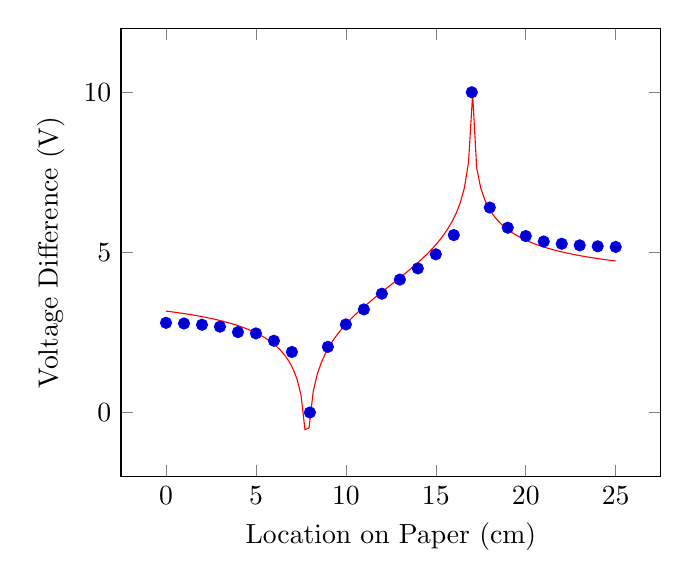
\begin{tikzpicture}
	\begin{axis}[xlabel={Location on Paper (cm)},
	ylabel = {Voltage Difference (V)},ymax=12,ymin=-2]
	\addplot+[only marks]
	table[]
	{
		x	y
		0	2.8
		1	2.78
		2	2.74
		3	2.68
		4	2.51
		5	2.47
		6	2.24
		7	1.89
		8	0
		9	2.05
		10	2.75
		11	3.22
		12	3.71
		13	4.15
		14	4.5
		15	4.94
		16	5.54
		17	10
		18	6.4
		19	5.77
		20	5.51
		21	5.34
		22	5.27
		23	5.22
		24	5.19
		25  5.17
	};
	\addplot[red,samples=111,domain=0:25] {1.016 * ln(abs((x-7.839)/(x-17.02)))+3.954};
	\end{axis}
	\end{tikzpicture}
\end{figure}
This fit is rather refreshingly better than the previous one. The \(\mathrm{R}\) is a substantial 99.2\%, and the RMSE is nearly of a third of the previous fit at 0.27 V. We can be rather confident that it makes more sense to model the dipole configuration as a set of oppositely charged parallel lines as opposed to two point charges. The parameters relay a similar story. The peaks of the function,\(a\) and \(b\) were predicted to be \(7.83 \pm 0.05\) cm and \(17.02 \pm 0.01\) cm. These are relatively closer to the true positions than the previous fit. Once again the leftmost point \(a\) is predicted to be father left than it truly is, perhaps the pin was not particularly well centered on its grid mark. The middle voltage was found to be \(3.95 \pm 0.05\) V, which is close to the voltage measured at the middle point \(3.93 \) V but once again distant from the assumed 5 V. This follows from the same explanation as before. The constant \(C\) represents \(2 k \lambda\) rather than \(q k \) as before. If we assume the dielectric constant of the carbon coated paper to be \(2.5 \pm 0.5\). We conclude that \(\lambda\), the linear charge density,to be \(1.4 \times 10^{-10} \pm 0.3 \times 10^{-11}\)  \(\mathrm{C}/m\)

If one uses this estimate for the linear charge density and the charge estimate found earlier, one can attempt to find the length of the parallel rod.
\begin{equation}
l = \frac{q}{\lambda}
\end{equation}
Dividing these two yields an estimate for line length of \(3.9 \pm 1.2 \)cm. The value for this is incredibility rough but it is about the length of the pin and alligator clip attached to the paper.

\subsection{Equipotentials and Field Lines}
The lines of equipotential were traced on copies of the gridded paper. These lines of equipotential were traced in green. One would expect the equipotentials of the dipole to take the characteristics of \textbf{(FIG 1)}. However, the measured potentials seem to extend father outward when outside of the dipole than they do in the model. This is because the dipole is better modeled by the parallel line fit. A logarithm is involved in the parallel line fit and thus it should die away much more slowly than standard dipole fit.
\begin{figure}[h]
	\begin{center}
		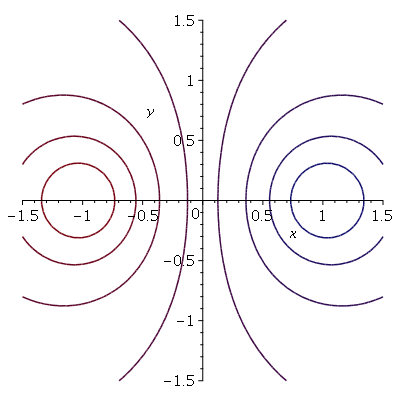
\includegraphics[width=2in]{cont}
		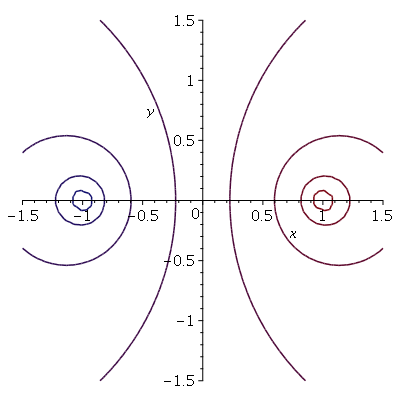
\includegraphics[width=2in]{ln}
	\end{center}
	\caption{ Contours of Electric potential for charge configurations. Dipole (Left) and Parallel Line (Right)}
\end{figure}
Notice how the contours traced much more closely match the parallel line fit, with much smaller curvature as contours get far away from the center.

An approximation of the field lines on the dipole has been drawn in red. Note that the red field lines always intersect perpendicular to green equipotentials and vice versa. Notice that the density of the field lines on the plane corresponds to the density of the equipotentials. That is, if there are many equi-potentials close to each other we expect the gradient of the electric potential to be large and thus we expect many field lines to pass through the area. This is well demonstrated at the center of the dipole. We also expect an equal number of field lines to pass into and out of each point (or any contour), as they have the same charge. This follows from Gauss' law which states that the electric flux through a surface is proportional to the charge enclosed. Because the charge for the two points is merely a sign change away, both will have an equal number of lines passing through, but one will that many field lines entering while the other will have that many leaving.

\subsection{Alternate Equipotentials}
The second configuration has similar characteristics. The field lines also cross perpendicular to the measured equipotentials as they would in any other diagram of field lines and equipotential. Ultimately this configuration will look like a dipole from a distance as it is comprised of a relatively compact pair of positively and negatively charged particles. Locally it is a bit more complicated than the dipole. At some points there were issues with some mal-connectivity. This explains the intersection of the green equipotential and the blue charge configuration at (5,12). In fact the very end of the charge configuration was not attached at all. One might also assume that there exists some larger accumulation of charge at the ends of the line and at the corner of the tear drop. This is not immediately evident but it may be occurring.
\end{document}